\section*{Цель}

Исследование характеристик процессов восстановления.

\section*{Порядок выполнения}

\begin{enumerate}
    \item Разработать программу для моделирования процесса восстановления.
    На экран в каждом прогоне модели выводить процесс восстановления, по результатам серии прогонов модели выводить
    графики функции восстановления $H(t)$, функции плотности вероятности $f(t)$, функции распределения $F(t)$,
    функции надежности $G(t)$ и функции опасности отказа $\phi(t)$.
    \item Исследовать поведение процесса восстановления для случайных величин \{$\xi_n$\}, имеющих распределение Вейбулла
    с заданными значениями параметров.
    Экспериментально с пятипроцентной точностью определить значения математического ожидания и дисперсии случайных
    величин \{$\xi_n$\}, значения функции восстановления $H(t)$, функции плотности вероятности $f(t)$, функции
    распределения $F(t)$, функции надежности $G(t)$ и функции опасности отказа $\phi(t)$.
    \item Рассчитать теоретические значения математического ожидания и дисперсии случайных величин \{$\xi_n$\},
    значения функции восстановления $H(t)$, функции плотности вероятности $f(t)$, функции распределения $F(t)$,
    функции надежности $G(t)$ и функции опасности отказа $\phi(t)$.
    Сравнить теоретические значения с экспериментальными.
    \item Классифицировать смоделированные процессы восстановления по функции опасности отказа.
\end{enumerate}

\section*{Исходные данные}

Заданы пары параметров $\alpha$ и $\lambda$, соответствующие трем моделям процесса восстановления.

\begin{align*}
    \alpha & = 1 & \alpha & = 0.1 & \alpha & = 2 \\
    \lambda & = 7 & \lambda & = 4 & \lambda & = 10
\end{align*}

\newpage

\section*{Диаграммы состояний}

Для каждой из моделей были построены диаграммы процесса восстановления $\eta(t)$ в рамках предварительных прогонов.

\begin{figure}[h!]
    \centering
    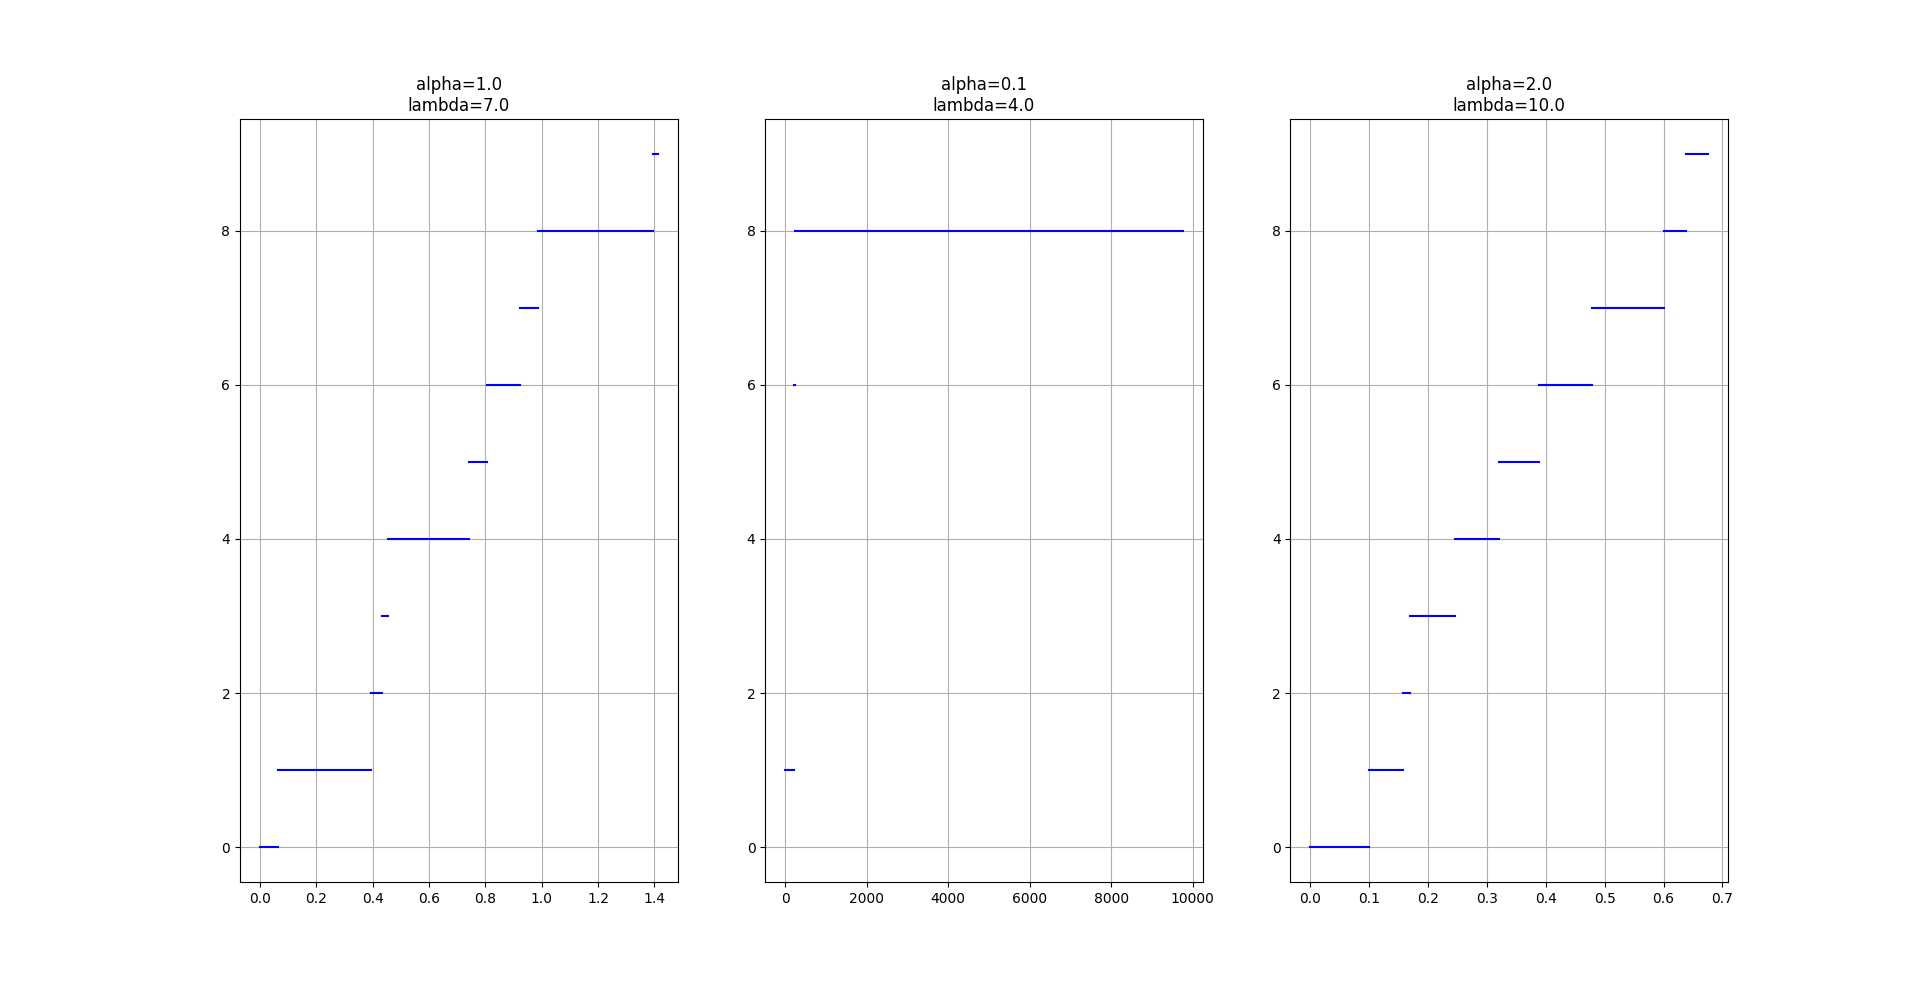
\includegraphics[width=\textwidth]{\jobname/docs/img/initial_diagrams.png}
    \caption{Диграммы процесса восстановления предварительных прогонов}
\end{figure}

\clearpage

\section*{Первая модель, $\alpha = 1, \lambda = 7$}

В качестве исследования заданной модели были произведены 1000 экспериментов с целью определения функции восстановления
$H(t)$, функции плотности вероятности $f(t)$, функции распределения $F(t)$, функции надежности $G(t)$ и функции
опасности отказа $\phi(t)$, а также с целью расчета значений математического ожидания и дисперсии
случайной величины \{$\xi_n$\}.

Значения экспериментальных  $M_e, D_e$ и теоретических $M_t, D_t$ значений математического ожидания и дисперсии
приведены далее.
Полученные графики функций восстановления, плотности вероятности, функции распределения, функции надежности и функции
опасности отказа также приведены ниже.

\begin{align*}
     M_e & = 0.14415 & D_e & = 0.01923 \\
     M_t & = 0.14286 & D_t & = 0.02041 \\
\end{align*}

\begin{figure}[h!]
    \centering
    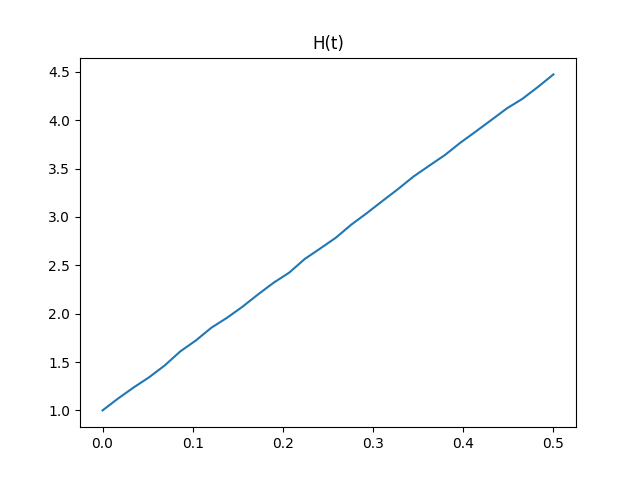
\includegraphics[width=\textwidth]{\jobname/docs/img/model-1_H.png}
    \caption{График функции восстановления первой модели}
\end{figure}

\begin{figure}[h!]
    \centering
    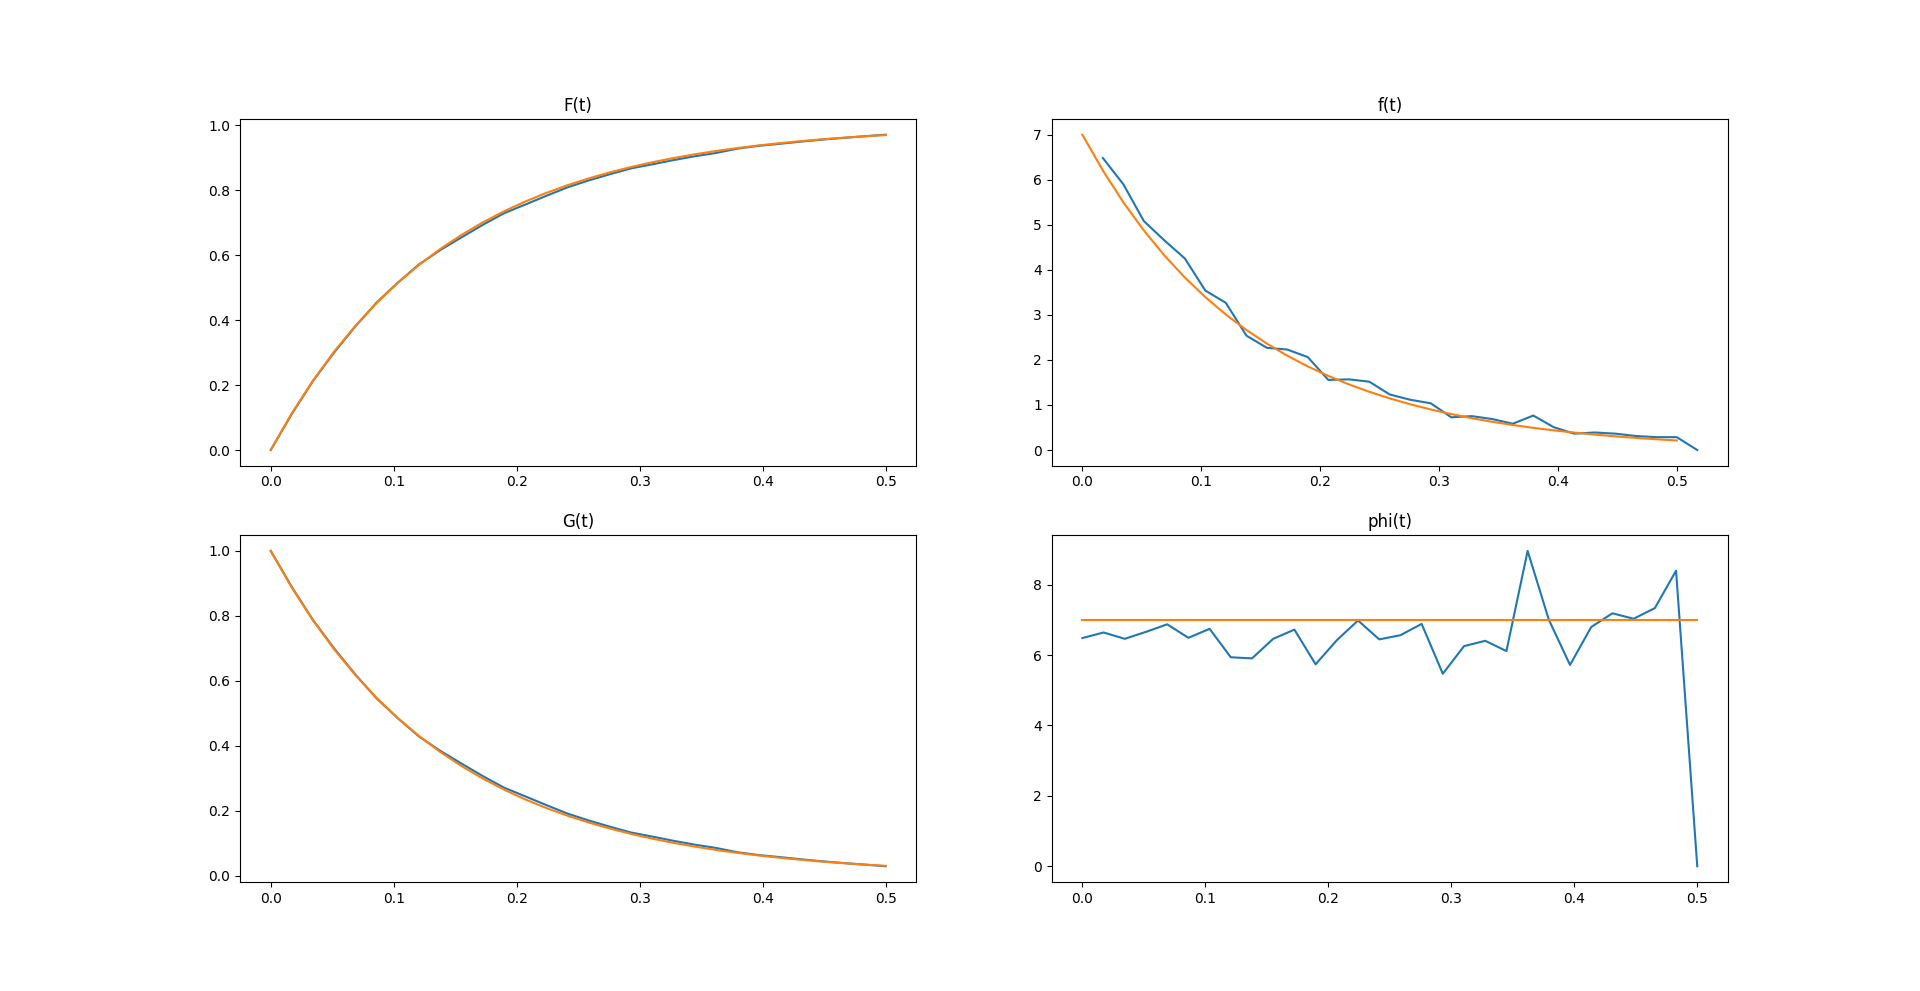
\includegraphics[width=\textwidth]{\jobname/docs/img/model-1_metrics.png}
    \caption{Графики функций восстановления, плотности вероятности, функции распределения, функции надежности и функции
    опасности отказа первой модели}
\end{figure}

\clearpage

\section*{Вторая модель, $\alpha = 0.1, \lambda = 4$}

В качестве исследования заданной модели были произведены 1000 экспериментов с целью определения функции восстановления
$H(t)$, функции плотности вероятности $f(t)$, функции распределения $F(t)$, функции надежности $G(t)$ и функции
опасности отказа $\phi(t)$, а также с целью расчета значений математического ожидания и дисперсии
случайной величины \{$\xi_n$\}.

Значения экспериментальных  $M_e, D_e$ и теоретических $M_t, D_t$ значений математического ожидания и дисперсии
приведены далее.
Полученные графики функций восстановления, плотности вероятности, функции распределения, функции надежности и функции
опасности отказа также приведены ниже.

\begin{align*}
     M_e & = 1.3 \cdot 10 ^ 6 & D_e & = 4.9 \cdot 10 ^ {15} \\
     M_t & = 0.9 \cdot 10 ^ 6 & D_t & = 152.1 \cdot 10 ^ {15} \\
\end{align*}

\begin{figure}[h!]
    \centering
    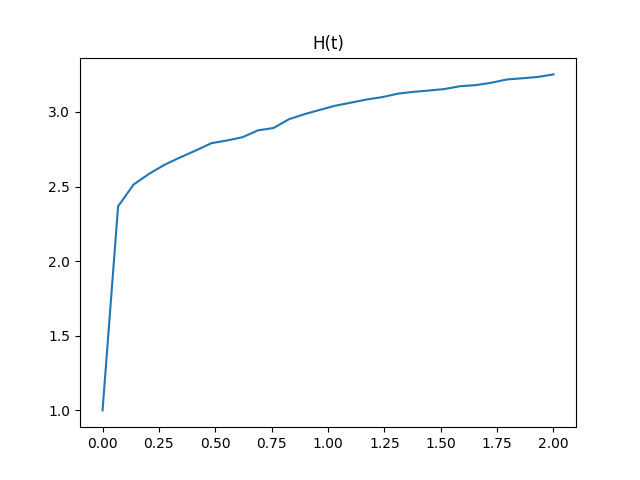
\includegraphics[width=\textwidth]{\jobname/docs/img/model-2_H.png}
    \caption{График функции восстановления второй модели}
\end{figure}

\begin{figure}[h!]
    \centering
    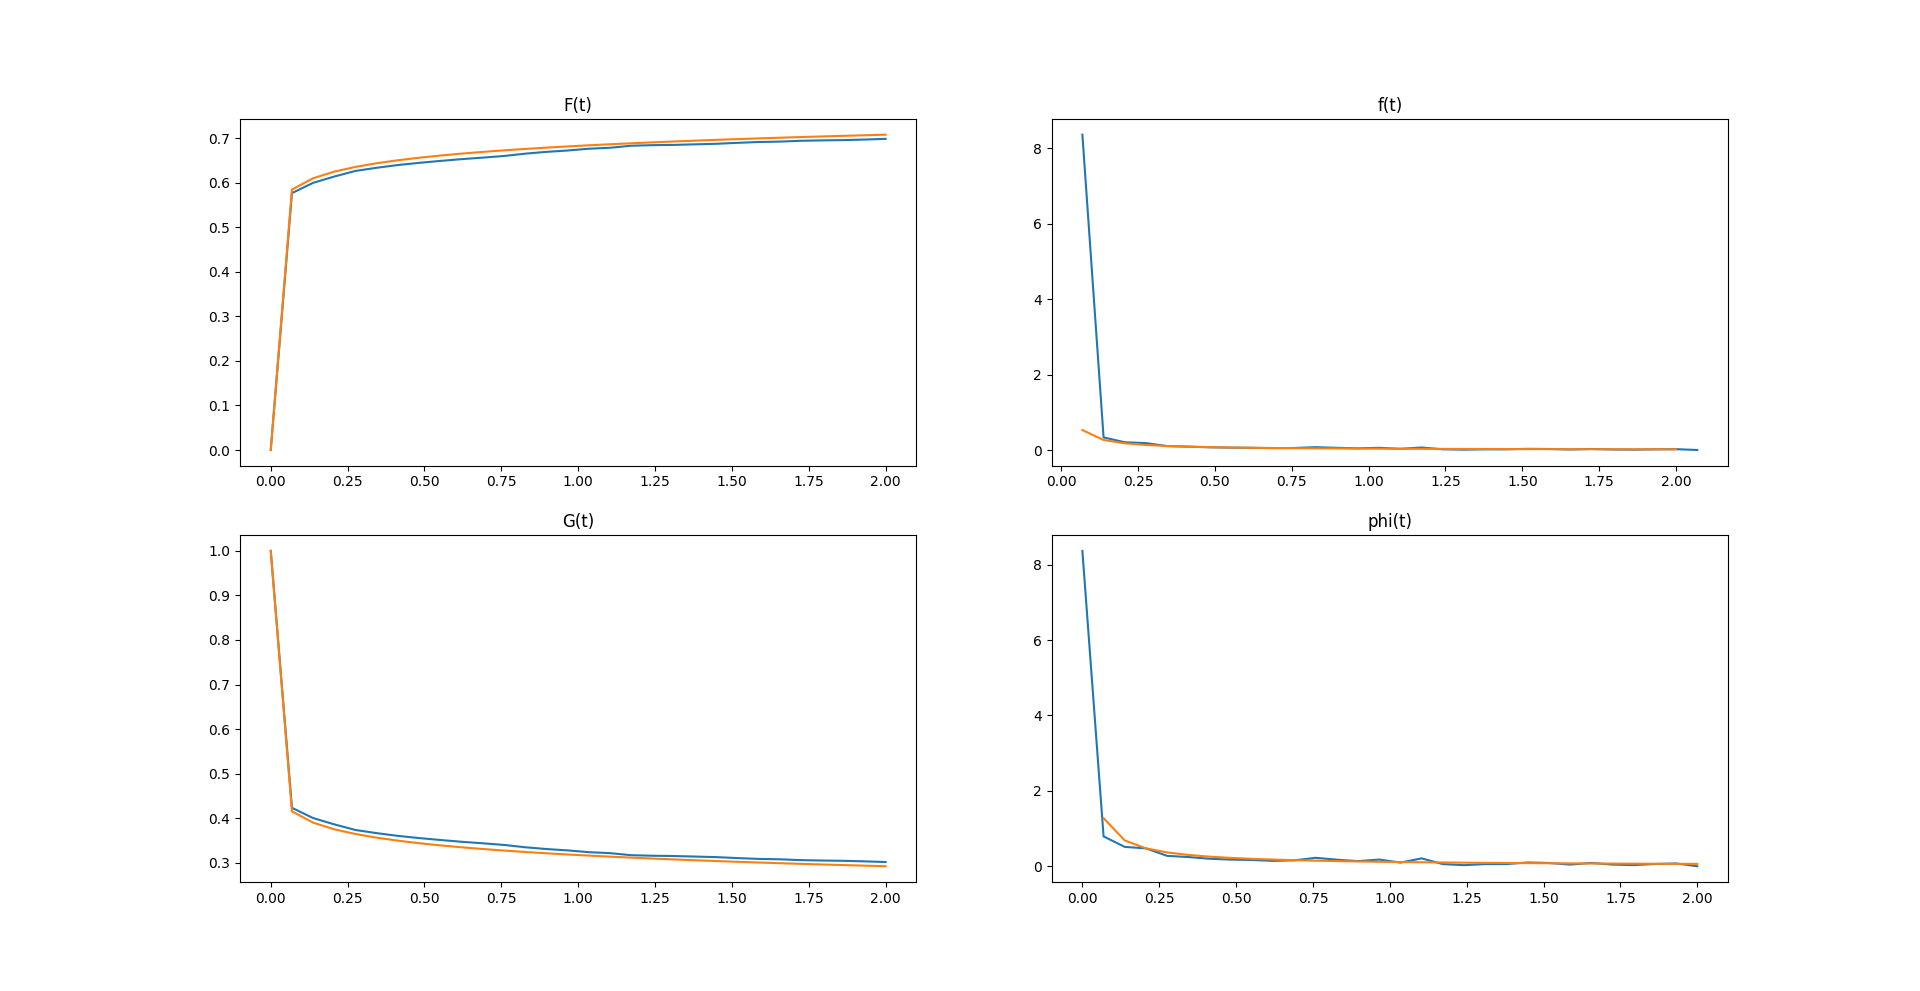
\includegraphics[width=\textwidth]{\jobname/docs/img/model-2_metrics.png}
    \caption{Графики функций восстановления, плотности вероятности, функции распределения, функции надежности и функции
    опасности отказа второй модели}
\end{figure}

\clearpage

\section*{Третья модель, $\alpha = 2, \lambda = 10$}

В качестве исследования заданной модели были произведены 1000 экспериментов с целью определения функции восстановления
$H(t)$, функции плотности вероятности $f(t)$, функции распределения $F(t)$, функции надежности $G(t)$ и функции
опасности отказа $\phi(t)$, а также с целью расчета значений математического ожидания и дисперсии
случайной величины \{$\xi_n$\}.

Значения экспериментальных  $M_e, D_e$ и теоретических $M_t, D_t$ значений математического ожидания и дисперсии
приведены далее.
Полученные графики функций восстановления, плотности вероятности, функции распределения, функции надежности и функции
опасности отказа также приведены ниже.

\begin{align*}
     M_e & = 0.08949 & D_e & = 0.00217 \\
     M_t & = 0.08862 & D_t & = 0.00215 \\
\end{align*}

\begin{figure}[h!]
    \centering
    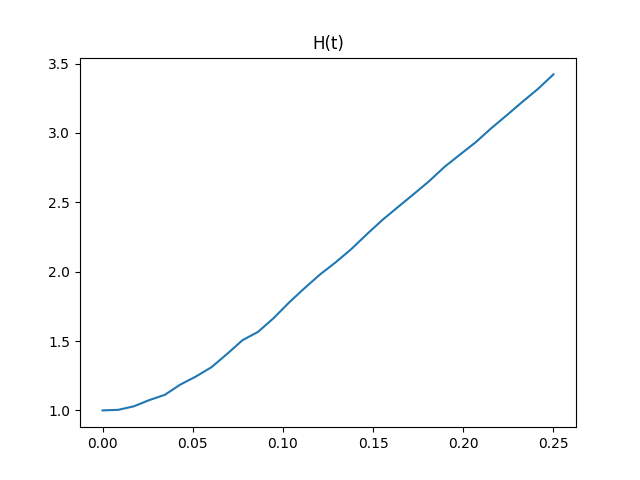
\includegraphics[width=\textwidth]{\jobname/docs/img/model-3_H.png}
    \caption{График функции восстановления третьей модели}
\end{figure}

\begin{figure}[h!]
    \centering
    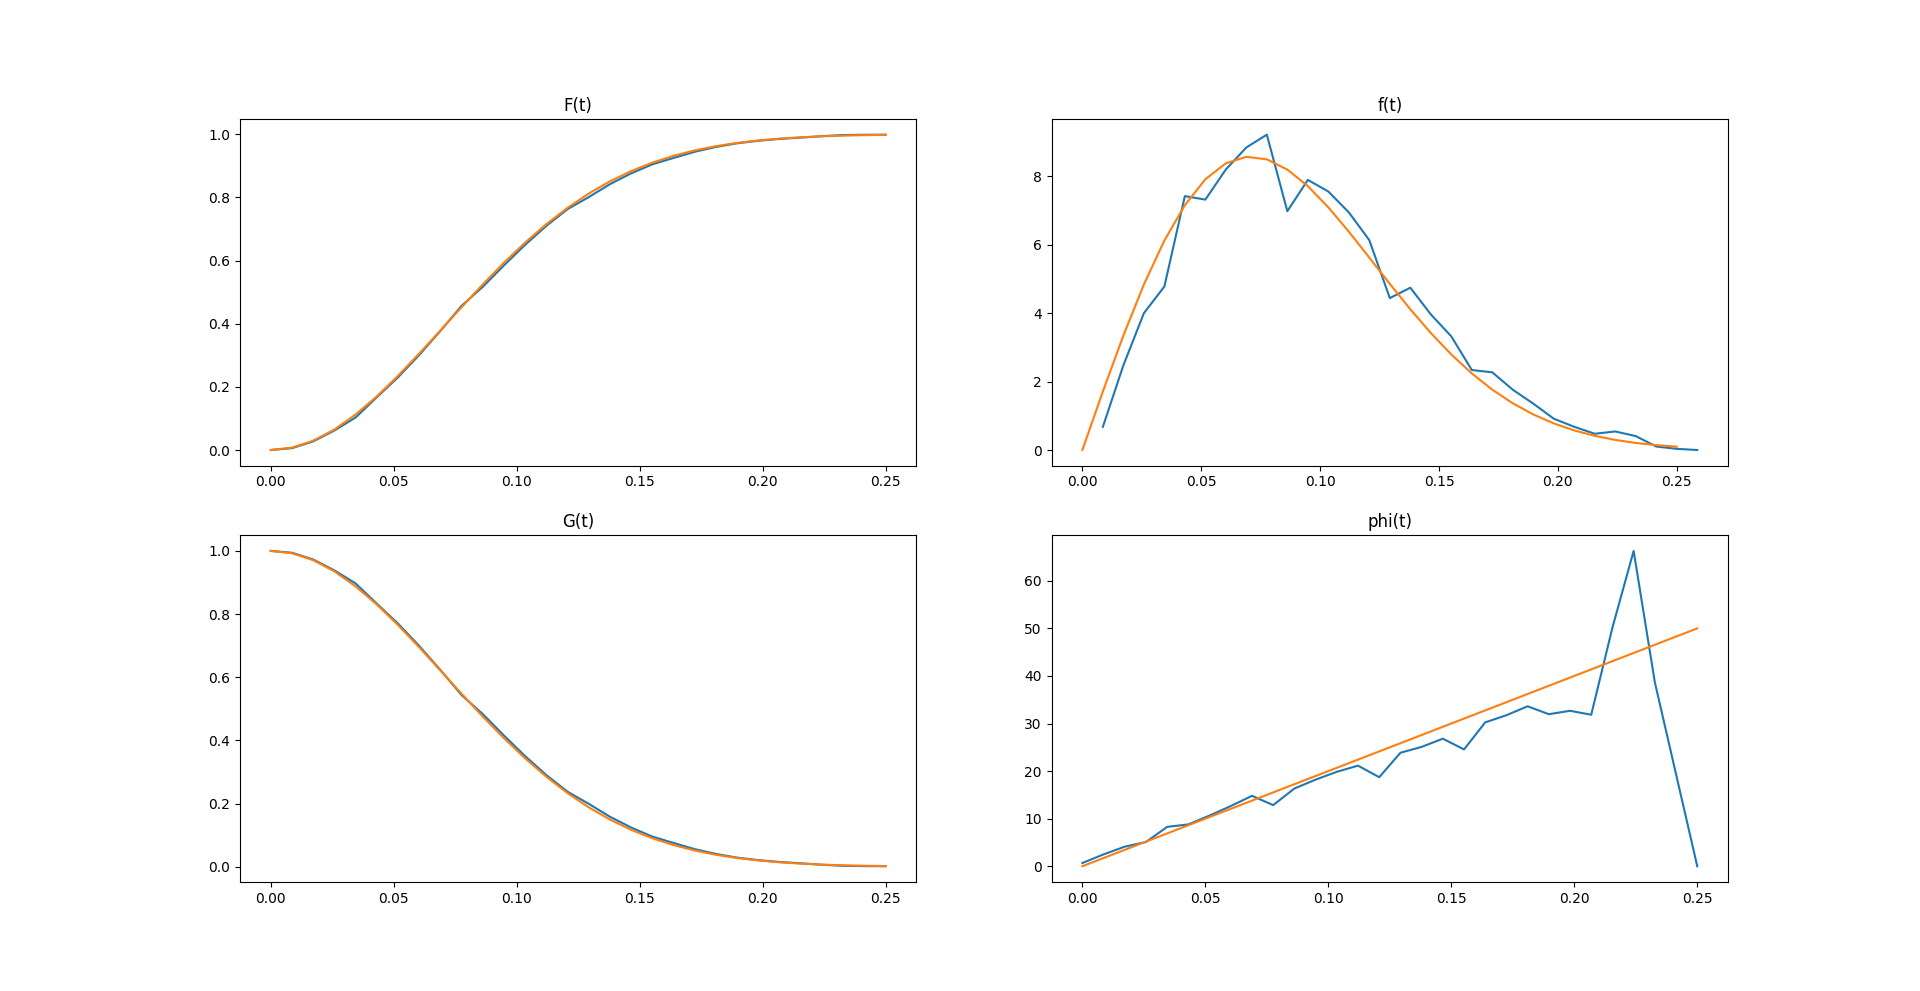
\includegraphics[width=\textwidth]{\jobname/docs/img/model-3_metrics.png}
    \caption{Графики функций восстановления, плотности вероятности, функции распределения, функции надежности и функции
    опасности отказа третьей модели}
\end{figure}

\clearpage

\section*{Выводы}

В ходе выполнения лабораторной работы были исследованы три процесса восстановления, заданные парами значений
параметров $\alpha$ и $\lambda$.
Для каждой из моделей были построены диаграммы процесса восстановления и графики функций восстановления,
плотности вероятности, функции распределения, функции надежности и функции опасности отказа.
Кроме того, были определены экспериментальные и теоретические значения математического ожидания и дисперсии.
Далее для каждой из моделей приведена классификации по признаку наличия старения и его вида - положительного или
отрицательного старения.

\subsection*{Первая модель}

На основании полученной функци опасности отказа, можно сделать вывод о том, что первая модель не отображает признаков
положительного или отрицательного старения.

\subsection*{Вторая модель}

На основании полученной функци опасности отказа, можно сделать вывод о том, что вторая модель отображает признаки
\textit{отрицательного} старения.

\subsection*{Третья модель}

На основании полученной функци опасности отказа, можно сделать вывод о том, что третья модель отображает признаки
\textit{положительного} старения.

\clearpage

\section*{Листинги}

\subsection*{Листинг основного скрипта}
\lstinputlisting[language=Python,texcl=true]{\jobname/lab.py}

\subsection*{Листинг скрипта, содержащего модель восстановления}
\lstinputlisting[language=Python,texcl=true]{\jobname/recovery.py}

\subsection*{Листинг скрипта, содержащего генераторы}
\lstinputlisting[language=Python,texcl=true]{\jobname/../common/gen.py}

\subsection*{Листинг скрипта, содержащего утилиты}
\lstinputlisting[language=Python,texcl=true]{\jobname/../common/utils.py}

\subsection*{Листинг скрипта, инициализируещего логирование}
\lstinputlisting[language=Python,texcl=true]{\jobname/../common/log.py}
